\chapter{Dynamic traffic assignment}

The purpose of AVDTA is to solve DTA with AVs, and the ``DTA'' tab contains options for loading and creating assignments. (An \textit{assignment} determine the route each vehicle takes.) Currently, AVDTA uses the method of successive averages to find an UE assignment. 

When a project is opened, no assignment is loaded by default. The \texttt{assignments} folder contains all previously stored assignments. Every time MSA is run, AVDTA will store the last iteration as a new assignment. Assignments are created with a random number as the name. However, assignments can be renamed as follows: Each assignment is a subfolder in the \texttt{assignments} folder. Renaming the subfolder will rename the assignment.

The AVDTA GUI provides a list of all existing assignments:
\begin{center}
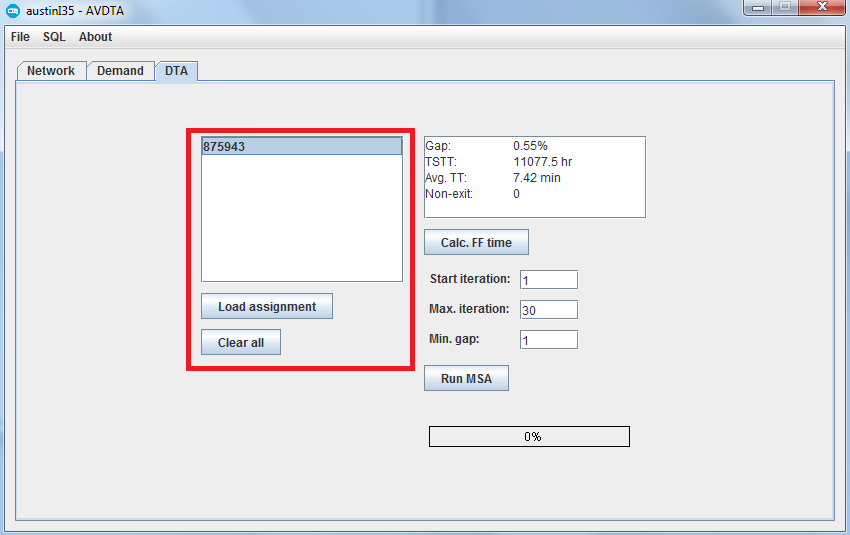
\includegraphics[width=0.8\textwidth]{images/msa2.png}
\end{center}
Selecting an assignment will fill the text area on the right with some summary statistics.
\begin{center}
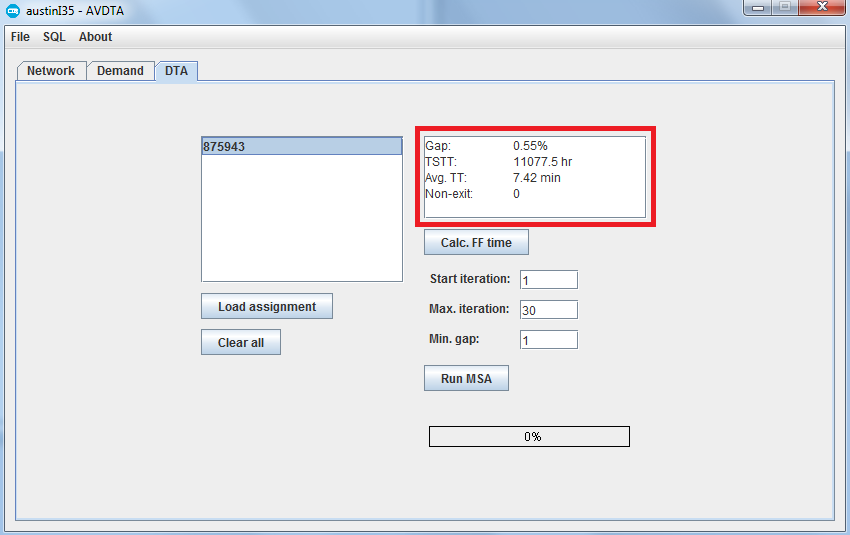
\includegraphics[width=0.8\textwidth]{images/msa3.png}
\end{center}
Clicking ``Load assignment'' will assign vehicles to the selected assignment.

Options to run MSA are on the right hand side. The starting iteration controls the initial step size ($\lambda=\frac{1}{i}$). When working with a previous assignment, it may be helpful to start at a lower step size. The stopping criteria are the maximum number of iterations and minimum gap. If either is reached, MSA will stop.
\begin{center}
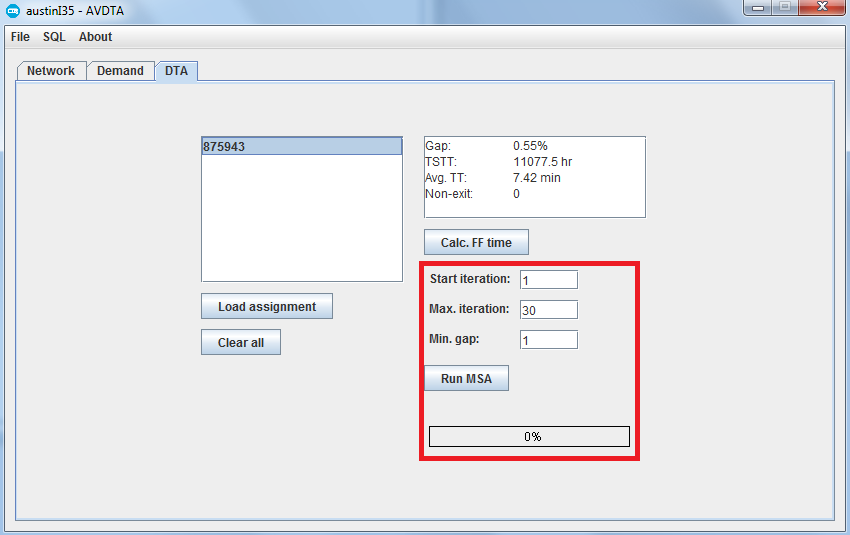
\includegraphics[width=0.8\textwidth]{images/msa1.png}
\end{center}
The status bar will estimate the completion and remaining time, based on computation time for previous iterations and the stopping criteria of the maximum number of iterations.